\chapter{Evaluation and Functional Validation}
\label{chap:validation}

\section{Evaluation scope}

This chapter evaluates whether the implemented system satisfies the declared thesis scope.
The focus is practical and reproducible validation, not exhaustive benchmarking of the entire SVG standard.

Validation targets three areas:

\begin{itemize}
\item parser correctness for representative inputs,
\item style normalization correctness,
\item executable proof of core functionalities F1 and F2.
\end{itemize}

\section{Methodology}

Evaluation is organized in three layers:

\begin{enumerate}
\item \textbf{Unit-level checks}: parser and color conversion tests.
\item \textbf{Functional checks}: dedicated F1 suite for path parse pipeline and F2 checks for color/style normalization.
\item \textbf{Scenario checks}: interactive verification in playground using simple and complex examples.
\end{enumerate}

This layered approach provides both precision (automated assertions) and practical confidence (integration behavior).
The class/layer interactions behind these two functions are shown in Figures~\ref{fig:f1_architecture} and~\ref{fig:f2_architecture}.
Those diagrams clarify that the tests do not validate isolated strings only; they validate the architectural boundaries that feed later geometry and rendering stages.

\section{Laboratory deliverable coverage}

The following matrix summarizes how the paper content addresses the staged laboratory requirements.
It is included explicitly to avoid relying on implicit chapter structure during evaluation.

\begin{table}[htbp]
\centering
\caption{Coverage of laboratory deliverables}
\label{tab:laboratory_deliverable_coverage}
\begin{tabular}{>{\raggedright\arraybackslash}p{2.0cm} >{\raggedright\arraybackslash}p{5.4cm} >{\raggedright\arraybackslash}p{5.4cm}}
\toprule
\textbf{Laboratory} & \textbf{Requirement} & \textbf{Where it is addressed} \\
\midrule
Lab 3 & thesis content; theoretical chapters with 2--3 subsections & Chapters~\ref{chap:svg_foundations} and~\ref{chap:geometry_conversion}, each with multiple theoretical sections/subsections \\
Lab 4 & Chapter 2 theoretical content with references, tables, images; practical requirements and specification & Chapter~\ref{chap:svg_foundations} includes references, tables, and figures; Chapter~\ref{chap:system_design} includes project specification, requirements, and architecture \\
Lab 5 & practical design, implementation, testing for F1; GUI interface; executable F1; mini-user manual and screen capture & Chapter~\ref{chap:system_design} covers design/implementation and Figure~\ref{fig:f1_architecture}; this chapter covers F1 tests, playground screenshots, and mini-user manual \\
Lab 6 & abstract, introduction, executable F2 & Abstract page, Chapter~\ref{chap:introduction}, Figure~\ref{fig:f2_architecture}, and automated F2 validation in this chapter \\
\bottomrule
\end{tabular}
\end{table}

\section{Execution context}

Tests are executed in the library package using Jest-based scripts.
The client playground is used for scenario-level verification and visual inspection.

\begin{table}[htbp]
\centering
\caption{Validation context}
\label{tab:validation_context_compact}
\begin{tabular}{>{\raggedright\arraybackslash}p{4.2cm} >{\raggedright\arraybackslash}p{8.4cm}}
\toprule
\textbf{Dimension} & \textbf{Context} \\
\midrule
Core package & \texttt{svg2gpu} \\
Test runner & Jest via npm scripts \\
Primary functional targets & F1 (SVG parse pipeline), F2 (style/color normalization) \\
Interactive verification surface & client playground \\
API/documentation verification & TypeDoc output \\
\bottomrule
\end{tabular}
\end{table}

\section{F1 definition}

F1 is the parser-centric functionality required before geometry/render stages.
For path-based input, F1 must guarantee:

\begin{itemize}
\item command stream parsing into typed command objects,
\item normalized style extraction,
\item typed element output suitable for downstream rendering,
\item safe rejection of invalid path elements (e.g., missing \texttt{d}).
\end{itemize}

Architecturally, F1 covers the route shown in Figure~\ref{fig:f1_architecture}.
The test suite enters through the public \texttt{SVGParser} API and checks both direct path-command parsing and full SVG element parsing.
This means F1 validates the conversion boundary from SVG path syntax to typed internal structures.

\section{Automated F1 validation}

\subsection{Test matrix}

\begin{table}[htbp]
\centering
\caption{Functional test cases for F1}
\label{tab:f1_matrix_compact}
\begin{tabular}{>{\raggedright\arraybackslash}p{1.8cm} >{\raggedright\arraybackslash}p{4.0cm} >{\raggedright\arraybackslash}p{6.6cm}}
\toprule
\textbf{Case} & \textbf{Input} & \textbf{Expected result} \\
\midrule
F1-T1 & path command string & typed command sequence in deterministic order \\
F1-T2 & valid SVG path with style & parsed path element with normalized style values \\
F1-T3 & invalid path without \texttt{d} & safe rejection (empty parsed result for invalid element) \\
\bottomrule
\end{tabular}
\end{table}

\subsection{Executable command}

\begin{verbatim}
cd svg2gpu && npm run test:f1
\end{verbatim}

Observed result for this dedicated suite:

\begin{itemize}
\item status: \textbf{PASS},
\item tests: \textbf{3 passed, 3 total},
\item exit code: \textbf{0}.
\end{itemize}

This is direct executable evidence that F1 works under the declared contract.

\section{F2 definition}

F2 is the style-normalization functionality required so that parsed SVG data can be rendered consistently.
SVG permits multiple color syntaxes and style representations; render pipelines require numeric, canonical values.
For supported input, F2 must guarantee:

\begin{itemize}
\item conversion of hexadecimal, RGB/RGBA, HSL/HSLA, named colors, \texttt{transparent}, and \texttt{none} into RGBA values,
\item safe rejection of invalid color strings,
\item normalized fill and stroke values in parsed SVG elements,
\item stable defaults for missing optional style attributes.
\end{itemize}

\section{Automated F2 validation}

\subsection{Test matrix}

\begin{table}[htbp]
\centering
\caption{Functional test cases for F2}
\label{tab:f2_matrix}
\begin{tabular}{>{\raggedright\arraybackslash}p{1.8cm} >{\raggedright\arraybackslash}p{4.0cm} >{\raggedright\arraybackslash}p{6.6cm}}
\toprule
\textbf{Case} & \textbf{Input} & \textbf{Expected result} \\
\midrule
F2-T1 & \texttt{\#00FF33} and short hex variants & normalized RGBA values in range $[0,1]$ \\
F2-T2 & \texttt{rgb()}, \texttt{rgba()}, \texttt{hsl()}, \texttt{hsla()} & equivalent canonical RGBA values \\
F2-T3 & named colors, \texttt{transparent}, \texttt{none} & recognized values mapped to RGBA output \\
F2-T4 & invalid color strings & safe rejection using \texttt{undefined} result \\
\bottomrule
\end{tabular}
\end{table}

\subsection{Executable command}

\begin{verbatim}
cd svg2gpu && npx jest --runInBand tests/color-parser/color.test.ts
\end{verbatim}

Observed result for this suite:

\begin{itemize}
\item status: \textbf{PASS},
\item tests: \textbf{21 passed, 21 total},
\item exit code: \textbf{0}.
\end{itemize}

This validates the color-conversion part of F2 directly.
F2 is also exercised indirectly by F1-T2, where parsed SVG path elements are checked for normalized \texttt{fill}, \texttt{stroke}, and \texttt{strokeWidth} fields.
The architectural scope is shown in Figure~\ref{fig:f2_architecture}: \texttt{ColorParser} performs syntax recognition and numeric conversion, while \texttt{SVGParser} consumes that normalized output when constructing element style objects.

\subsection{Acceptance criteria for F1}

To avoid ambiguous interpretation, F1 validation is evaluated against explicit acceptance criteria:

\begin{itemize}
\item all dedicated F1 test cases pass in one execution,
\item parsed command sequences preserve deterministic order,
\item invalid mandatory path data is rejected safely,
\item normalized style fields are present for valid path elements.
\end{itemize}

These criteria focus on parser reliability and data integrity, because later conversion stages depend on this contract.
If F1 becomes non-deterministic, downstream geometry behavior cannot be trusted.

\begin{table}[htbp]
\centering
\caption{Acceptance criteria mapping for F1}
\label{tab:f1_acceptance_mapping}
\begin{tabular}{>{\raggedright\arraybackslash}p{3.6cm} >{\raggedright\arraybackslash}p{3.2cm} >{\raggedright\arraybackslash}p{5.8cm}}
\toprule
\textbf{Criterion} & \textbf{Status} & \textbf{Observed evidence} \\
\midrule
Command parse determinism & satisfied & stable typed sequence in F1-T1 \\
Style normalization presence & satisfied & normalized style object in F1-T2 \\
Invalid mandatory field handling & satisfied & safe rejection in F1-T3 \\
Executable run integrity & satisfied & pass status and zero exit code \\
\bottomrule
\end{tabular}
\end{table}

\subsection{Acceptance criteria for F2}

F2 validation is evaluated against the following criteria:

\begin{itemize}
\item all color parser tests pass in one execution,
\item supported color syntaxes are converted to normalized RGBA arrays,
\item \texttt{transparent} and \texttt{none} produce transparent RGBA output,
\item invalid color strings return \texttt{undefined},
\item parsed SVG elements receive usable defaults for missing optional style fields.
\end{itemize}

\begin{table}[htbp]
\centering
\caption{Acceptance criteria mapping for F2}
\label{tab:f2_acceptance_mapping}
\begin{tabular}{>{\raggedright\arraybackslash}p{3.8cm} >{\raggedright\arraybackslash}p{3.0cm} >{\raggedright\arraybackslash}p{5.8cm}}
\toprule
\textbf{Criterion} & \textbf{Status} & \textbf{Observed evidence} \\
\midrule
Hex/RGB/HSL conversion & satisfied & F2-T1 and F2-T2 color parser tests \\
Named color handling & satisfied & F2-T3 color parser tests \\
Transparent/none handling & satisfied & named color tests for transparent output \\
Invalid color rejection & satisfied & F2-T4 invalid input checks \\
Executable run integrity & satisfied & pass status and zero exit code \\
\bottomrule
\end{tabular}
\end{table}

\section{Reproducibility checklist}

To keep evaluation repeatable during review or defense, the following minimal checklist can be used:

\begin{enumerate}
\item enter the \texttt{svg2gpu} directory,
\item ensure dependencies are installed,
\item execute the F1 command,
\item execute the F2 command,
\item confirm pass status, test count, and zero exit code for both suites.
\end{enumerate}

This checklist intentionally avoids hidden configuration assumptions.
Its role is to ensure that the functional claim is independently verifiable.

\section{Scenario-level verification}

Simple scenes validate basic parser and style behavior quickly.
Complex scenes reveal robustness boundaries under dense input.
The Tiger SVG example is used as stress scenario.

\begin{figure}[htbp]
    \centering
    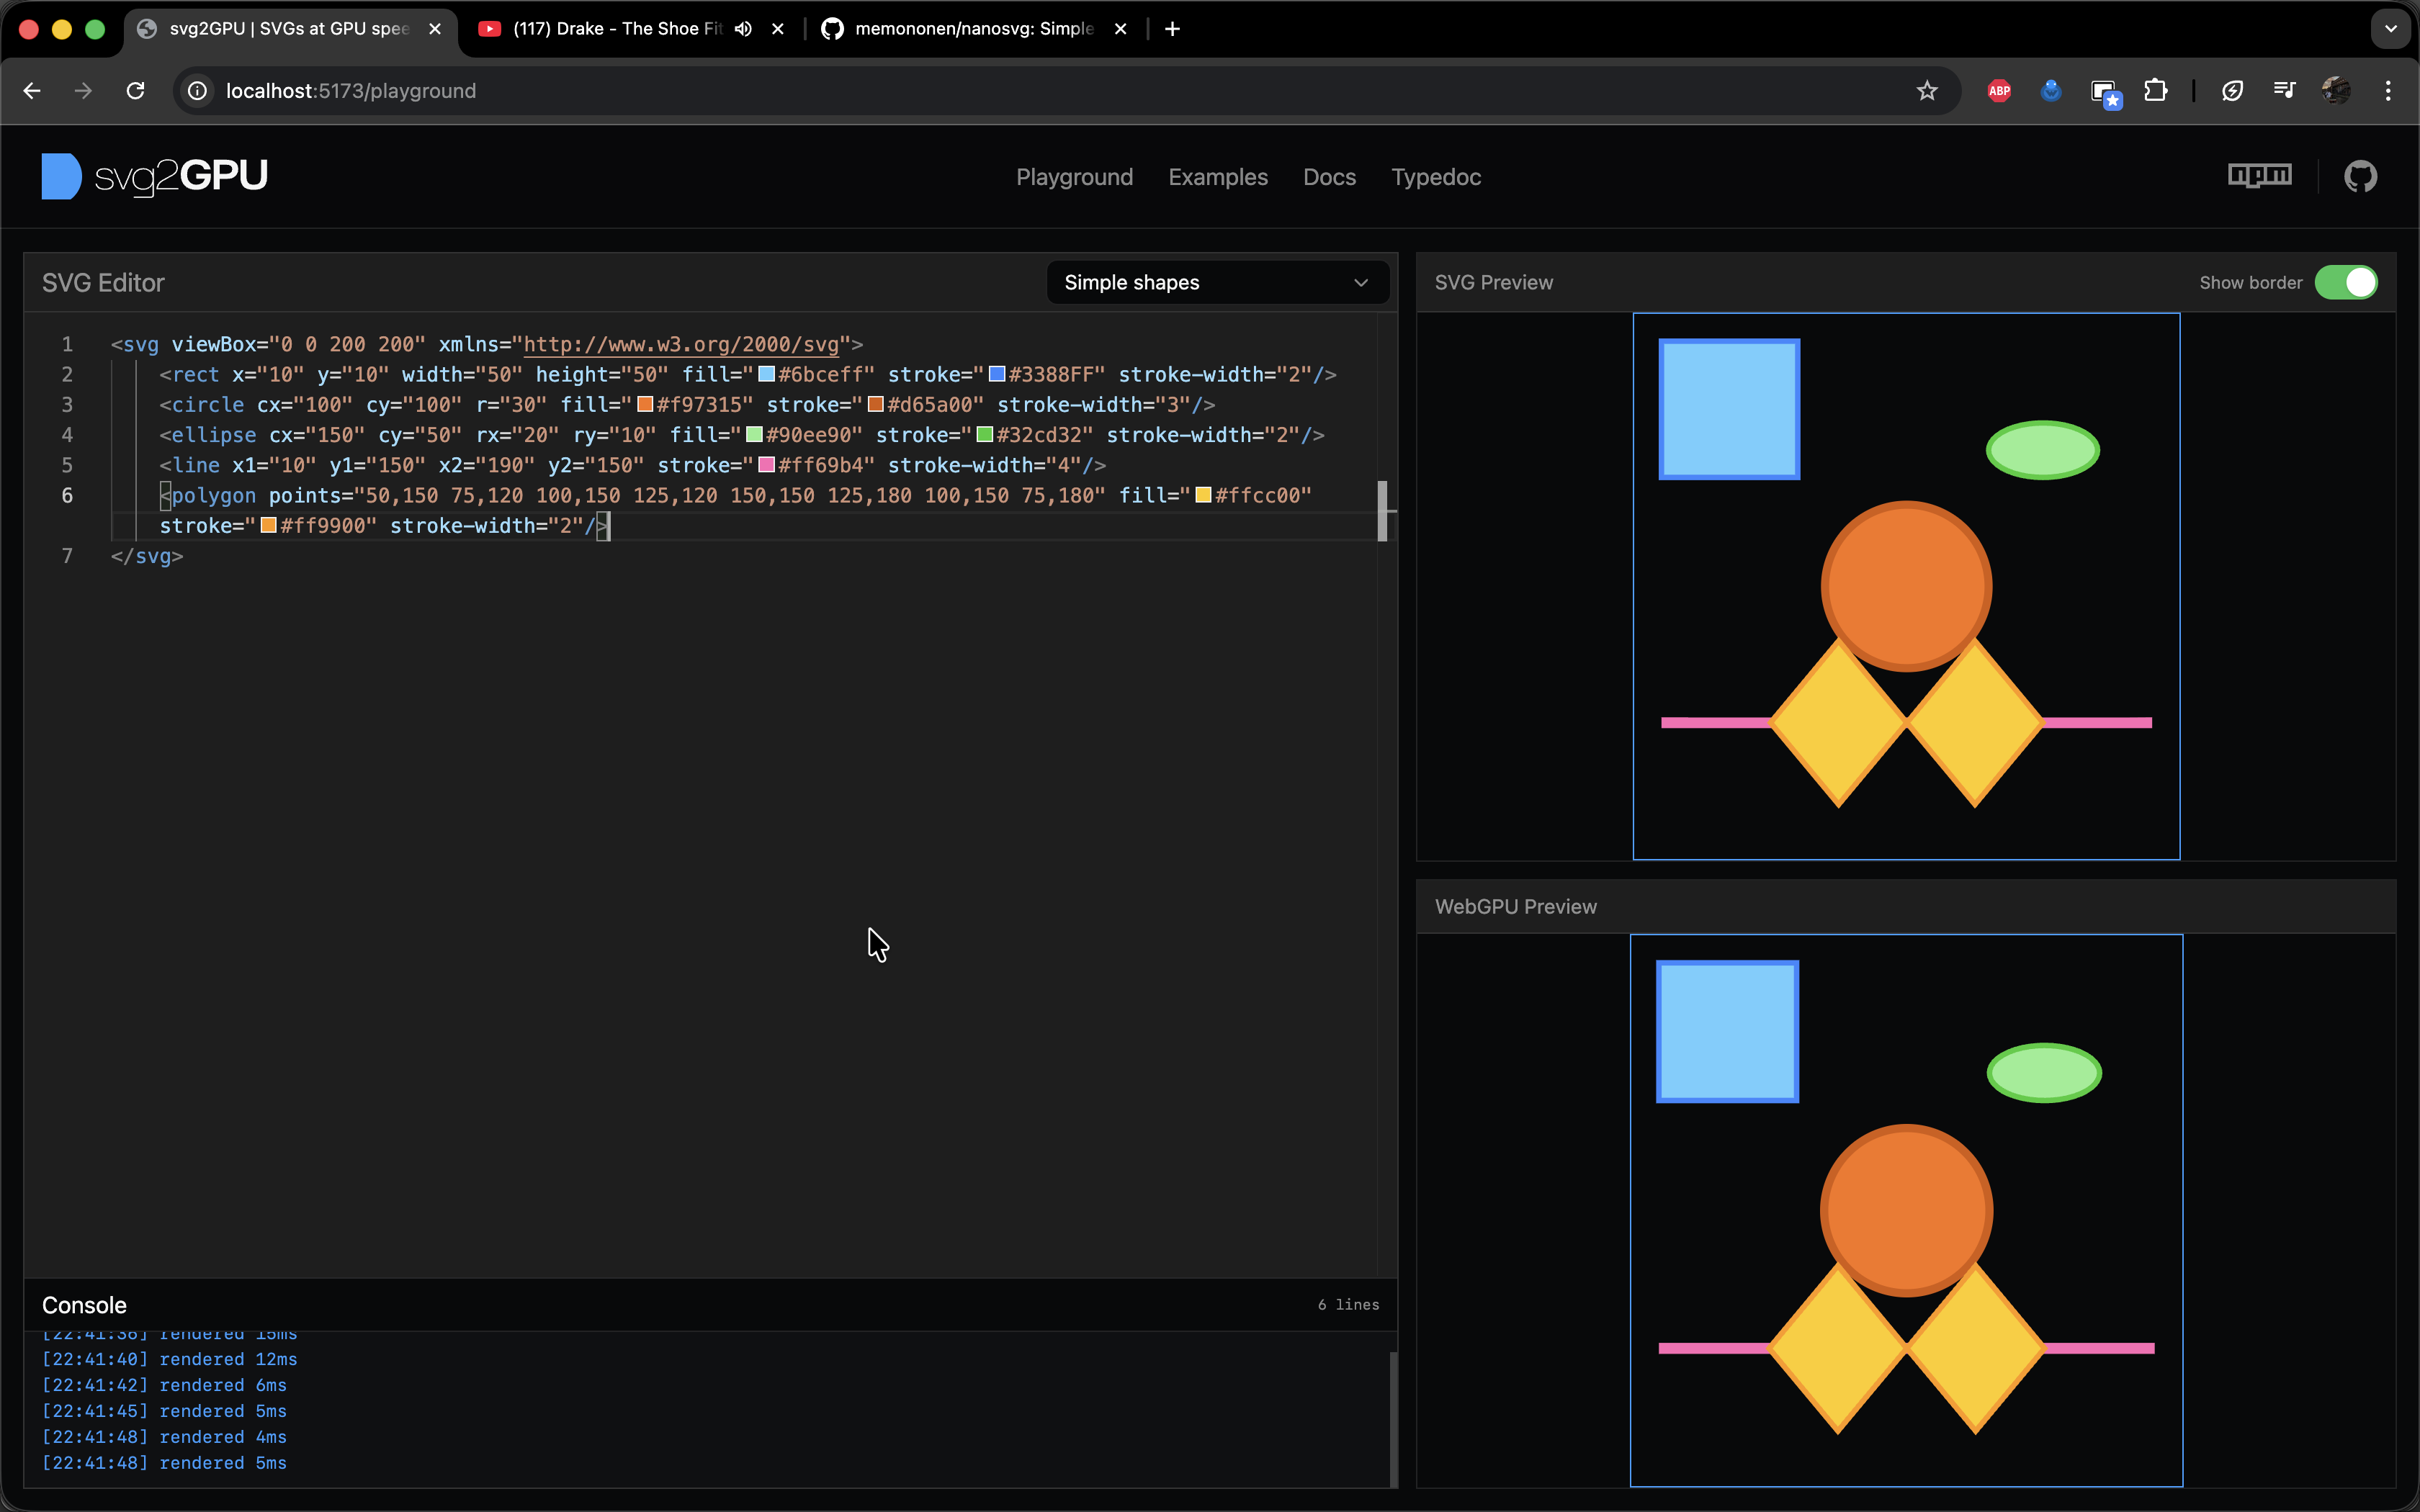
\includegraphics[width=0.92\textwidth]{figures/BasicGeometries.png}
    \caption{Playground execution with basic SVG geometry and visual preview}
    \label{fig:validation_basic_case}
\end{figure}

\begin{figure}[htbp]
    \centering
    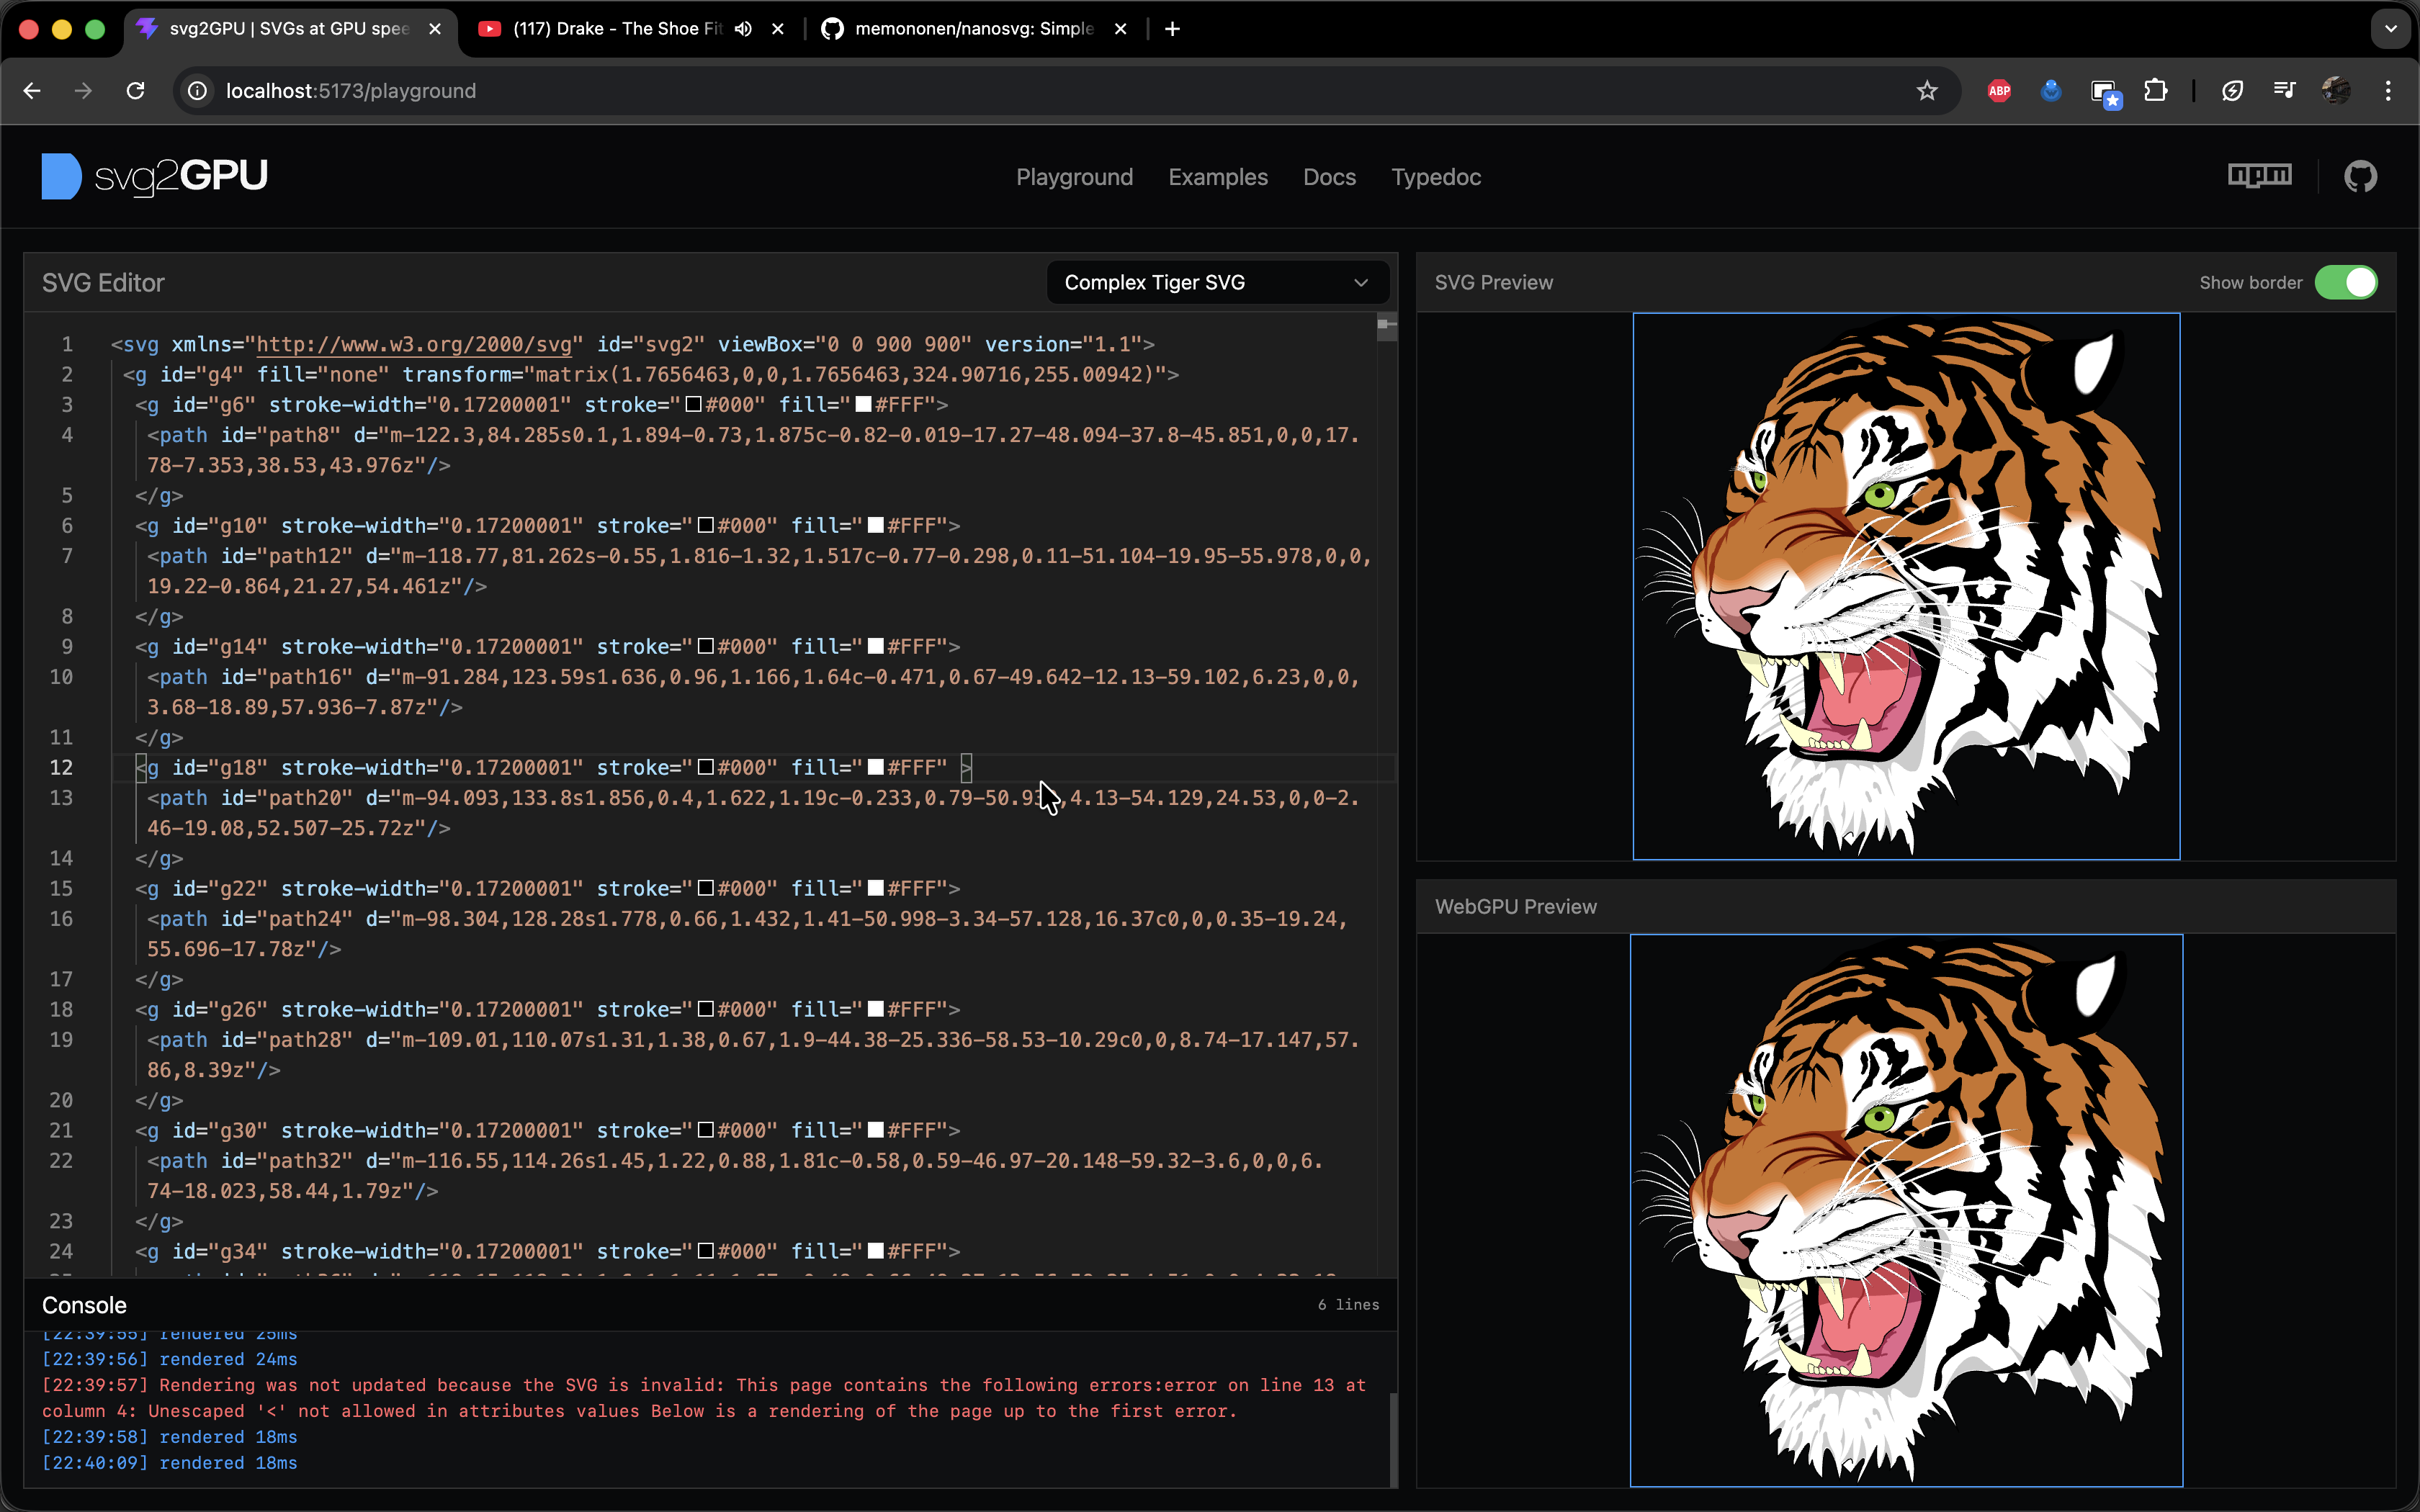
\includegraphics[width=0.92\textwidth]{figures/TigerSVG.png}
    \caption{Complex scenario used for integration-level stress observation}
    \label{fig:validation_complex_case}
\end{figure}

Scenario checks complement automated tests by exposing behavior under realistic content density.

\section{Mini-user manual for F1 and F2}

The following minimal procedure can be used by an evaluator to demonstrate the two implemented functionalities:

\begin{enumerate}
\item Install dependencies in the \texttt{svg2gpu} package if they are not already installed.
\item Run \texttt{npm run test:f1} to demonstrate F1, the SVG path parsing pipeline.
\item Run \texttt{npx jest --runInBand tests/color-parser/color.test.ts} to demonstrate F2, the color/style normalization pipeline.
\item Start the client playground and open a basic SVG example.
\item Edit a path command or style value, then observe that the preview and diagnostics update.
\item Compare the native SVG preview with the rendered/processed output for supported features.
\end{enumerate}

For F1, the evaluator should focus on whether valid path data becomes deterministic typed commands and whether invalid path data is rejected safely.
For F2, the evaluator should focus on whether different SVG color syntaxes produce consistent RGBA values and whether invalid colors are rejected instead of producing unstable renderer state.

\subsection{Observed scenario behavior}

In the controlled basic example, parser output and style interpretation remain stable across repeated edits.
This confirms that common inputs are handled with predictable behavior in the interactive environment.

In the complex example, the system continues to provide deterministic diagnostics and render output for supported features.
The stress scenario is useful mainly for identifying scope boundaries and potential future hardening targets rather than for claiming complete SVG parity.

\section{Result interpretation}

\subsection{Validated with high confidence}

\begin{itemize}
\item deterministic parsing for representative path inputs,
\item style normalization for supported formats,
\item safe rejection of invalid mandatory path data,
\item reproducible execution of dedicated F1 tests,
\item reproducible execution of F2 color-normalization tests.
\end{itemize}

\subsection{Partially validated or out of current scope}

\begin{itemize}
\item complete SVG feature parity,
\item full triangulation hardening for all pathological contours,
\item full benchmark suite across browsers/devices,
\item complete WebGPU-native parity.
\end{itemize}

These constraints are explicit and consistent with project scope.

\section{Threats to validity}

The main threats are:

\begin{itemize}
\item scope limitation to a supported SVG subset,
\item dependence on current toolchain/runtime,
\item finite scenario diversity.
\end{itemize}

Mitigation includes dedicated functional scripts, typed contracts, and modular architecture for incremental extension.

\section{Evaluation procedure for reproducibility}

For thesis review, the following procedure provides a consistent reproducibility path:

\begin{enumerate}
\item run the dedicated F1 test command and record status, test count, and exit code,
\item run the dedicated F2 color parser command and record status, test count, and exit code,
\item execute a controlled playground scenario with basic primitives and confirm stable behavior,
\item execute a complex scenario and record diagnostic output for unsupported or edge behaviors,
\item compare results with acceptance criteria from Tables~\ref{tab:f1_acceptance_mapping} and~\ref{tab:f2_acceptance_mapping}.
\end{enumerate}

This procedure links automated evidence with integration-level observation.
It also makes evaluation independent of implicit local knowledge, which is important for transparent academic assessment.

\section{Lessons learned from validation}

Validation produced several practical lessons that influence future development:

\begin{itemize}
\item focused functional scripts are easier to maintain and present than only broad test suites,
\item deterministic parser output dramatically reduces debugging complexity,
\item explicit scope boundaries improve credibility by avoiding overclaimed capabilities,
\item combining automated tests with scenario-level checks provides better confidence than either approach alone.
\end{itemize}

These lessons support the long-term sustainability of the project, especially when feature coverage is expanded.

\section{Evaluation summary}

\begin{table}[htbp]
\centering
\caption{Compact evaluation summary}
\label{tab:evaluation_summary_compact}
\begin{tabular}{>{\raggedright\arraybackslash}p{4.2cm} >{\raggedright\arraybackslash}p{3.0cm} >{\raggedright\arraybackslash}p{5.0cm}}
\toprule
\textbf{Criterion} & \textbf{Status} & \textbf{Evidence} \\
\midrule
F1 executable parser functionality & satisfied & dedicated test suite \texttt{test:f1} \\
F2 style/color normalization behavior & satisfied (supported formats) & \texttt{tests/color-parser/color.test.ts} \\
Safe invalid-path handling & satisfied & F1-T3 and parser guards \\
Interactive integration workflow & satisfied (prototype scope) & playground scenarios \\
API documentation availability & satisfied & TypeDoc output \\
\bottomrule
\end{tabular}
\end{table}

\section{Chapter summary}

Evaluation confirms that the implemented system meets its core functional goal for the selected scope.
The F1 and F2 executable tests provide clear reproducible evidence, while scenario checks support practical integration confidence.
The result is a validated baseline suitable for extension and optimization in future work.
